\chapter{Performance Evaluation}
\label{cha:evaluation}

Answering the question of the GC performance under a real-world setting,
this chapter discusses the performance evaluation I undertaken for analyzing
the Garbage-First family of garbage collectors. This chapter will firstly describe the software and hardware platform I used for benchmarking,
Then the detailed evaluation process and resutls of both pause time and
barrier latency will be presented and discussed.

Section~\ref{sec:dacapo} and \ref{sec:hardware} roughly introduce the experimental
platform and software involved for the performance measurements.
Section~\ref{sec:generalmethod} discusses the generall evaluation method used to
evaluate the performance of all the interested metrics.
Section~\ref{sec:pausetime}, \ref{sec:barrierlatency} and \ref{sec:remsetsize} discusses the detailed
measurement steps involved to evaluate the GC pause time, barrier overhead and remembered set size
respectivelt, as well
as figures of the results and the discussion based on the results.

\section{The Dacapo Benchmark} % 2
\label{sec:dacapo}

The Dacapo Benchmark Suite is a tool for Java benchmarking and contains a set of
open-sourced real world programs with a high memory loads.

The Dacapo Benchmark is frequently used during the development of the G1 family
of garbage collectors in chapter~\ref{cha:implementation}, as a validation program
to verify the correctness of the collectors under a real world setting.

I also performed pause time evacuations and barrier latency evaluation
on all of the following Dacapo Benchmark suites.
The benchmarking suites I used for evaluation includes (\cite{Blackburn:2006:DBJ:1167515.1167488}):

\begin{itemize}
  \item \textbf{luindex} Uses lucene to indexes a set of documents; the works of Shakespeare and the King James Bible
  \item \textbf{bloat} Performs a number of optimizations and analysis on Java bytecode files
  \item \textbf{hsqldb} Executes a JDBCbench-like in-memory benchmark, executing a number of transactions against a model of a banking application
  \item \textbf{lusearch} Uses lucene to do a text search of keywords over a corpus of data comprising the works of Shakespeare and the King James Bible
  \item \textbf{pmd} Analyzes a set of Java classes for a range of source code problems
  \item \textbf{xalan} Transforms XML documents into HTML
  \item \textbf{avrora} Simulates a number of programs run on a grid of AVR microcontrollers
  \item \textbf{sunflow} Renders a set of images using ray tracing
\end{itemize}

By performing evaluation on a wide range of benchmarking suites which represents different
class of real world programs, it is more possible to understand the pros and cons
of the G1 family of collectors under a real world setting.

\section{Hardware Platform} % 2
\label{sec:hardware}

During the implementation of all the G1 family of garbage collectors in chapter~\ref{cha:implementation},
a list of machine with a large varities on CPU types, clock, number of processors and
the size of cache and memory were involved, as shown in Table~\ref{tab:machines}.
By executing all the benchmarking suite of the Dacapo Benchmark on these different machines,
and thanks to the benchmarking suites of the Dacapo Benchmark which reflect
that different categories of programs in the real world,
we have the ability to statistically verify the correctness of the prevously
implemented garbage collectors (in chapter~\ref{cha:implementation})
and make sure they performs as intended in a real world setting.

For further performance evaluation, the "fisher" machine was used for the final benchmarking.

\begin{table*}
  \centering
  \input table/machines.tex
  \caption{Machines used for development and evaluation.}
  \label{tab:machines}
\end{table*}

\section{General Measurement Methodology}
\label{sec:generalmethod}

I perform both GC pause time and barrier overhead measurements on the optimized build
of the JikesRVM, with 6 different GC configurations for the 6 GCs to be measured respecively.
To collect measurement results, I execute all 10 dacapo benchmark suites discussed in section~\ref{sec:dacapo}
on all 6 collectors, with respect to 4 different heap sizes, 637\,MB, 939\,MB, 1414\,MB and 1971\,MB
respecively. Each benchmark suite is executed 10 times for each configuration of $(GC, HeapSize)$ to
collect more precise results and avoids the error due to some unexpected environmental fluctuations.

\subsection{Reducing non-determinisms}
\label{subsec:nondeterminisms}

The adaptive compiler can have non-deterministic behaviours when performing dynamic
compilations and optimizations to the executing Java program. In order to minimize
such non-deterministic behaviours and makes the program executes more faster, I performed
the measurement methodology called "warmup replay", which was firstly introduced by
\cite{yang2012barriers}, as a replacement of the "pseudoadaptive approach" introduced by \cite{blackburn2004barriers}.

This methodology performs a execution of 10 iterations for each benchmark suite to
collect runtime execution informations before the measurement, to assist with more optimized compilation.
Then during measurements, after the first iteration of warmups, JikesRVM compiles all
methods by using the advice information generated previously to avoid any re-compiling
behaviours buring the following measurement iteration.

I ran all of the 9 benchmark suites discussed in section~\ref{sec:dacapo} on each collector
for 10 times, with 2 times of warmup execution before the timing iteration.
JikesRVM performs warmup-replay compilation at the end of the first warmup iteration.

\section{Pause Time Evaluation} % 7
\label{sec:pausetime}

This section describes the steps took for pause time evaluation as well as
all the evaluation results and discussions.

\subsection{Mutator latency timer}

In order to perform more careful analysis on the mutator pause times, instead of
simply calculating the time starting from the first stop-the-world phase to the last
stop-the-world phase during each GC cycle, I implemented a mutator latency timer
to perform more precise calculation of mutator pause times.

The mutator latency timer contains a static "three dimemsional" array:\\
\centerline{\textjava{static long[] LOGS = long[THREAD ID * EVENT ID * TIMESTAMPS]}}
This array is statically allocated within the VM Space to record the timestamp (in nanoseconds)
of each event, for each mutator. The first dimension is the thread id of all
mutators. The second dimension is the event id. The third dimemsion \textjava{TIMESTAMPS} is the
max number of logs of one event and is currently set to $1024$. Particularly under
current context, to measure the pause time for each mutator, two events,
\textjava{MUTATOR_PAUSE} and \textjava{MUTATOR_RESUME} are defined to record the time when a
mutator thread starts waiting for gc complete and the time when a mutator gets resumed for execution.

In JikesRVM, a mutator thread checks for GC requests and starts waiting if necessary every
time it reaches a yieldpoint, which may trigger a \textjava{MUTATOR_PAUSE} event if it should
be paused. After a stop-the-world cycle is finished, before continuing for further execution,
it triggers a \textjava{MUTATOR_RESUME} event.

At the end of the benchmark execution, the mutator latency timer will dump all the
data in the \textjava{LOGS} array to the print buffer for further data analysis.

As an output of the analysis of the overhead data, I report the minimun, 25\%, 50\%,
75\% and maximum mutator pause time for each GC, each benchmark suite and each heap size.

\subsection{MMTk harness callbacks}

During each iteration of benchmarking, the Dacapo benchmark has several warm-up
executions which will run the benchmark suite a few times to warm up the cache and JVM.
Then dacapo will starts the actual benchmarking run. I use a probe called \textjava{MMTKCallback}
which will call the \textjava{org.mmtk.plan.Plan.harnessBegin} method
before the final benchmarking execution and call the \textjava{org.mmtk.plan.Plan.harnessEnd}
after the final benchmarking execution. Based on this, the two callbacks
\textjava{harnessBegin} and \textjava{harnessEnd} are used to calculate the inform the mutator
latency timer to start recording logs or dump all logs.

\subsection{Results}

\begin{table*}
  \centering
  \label{tab:pause}
  \input table/average-pause.tex
  \caption{Results of the GC pause time}
\end{table*}

\begin{figure*}
  \centering
  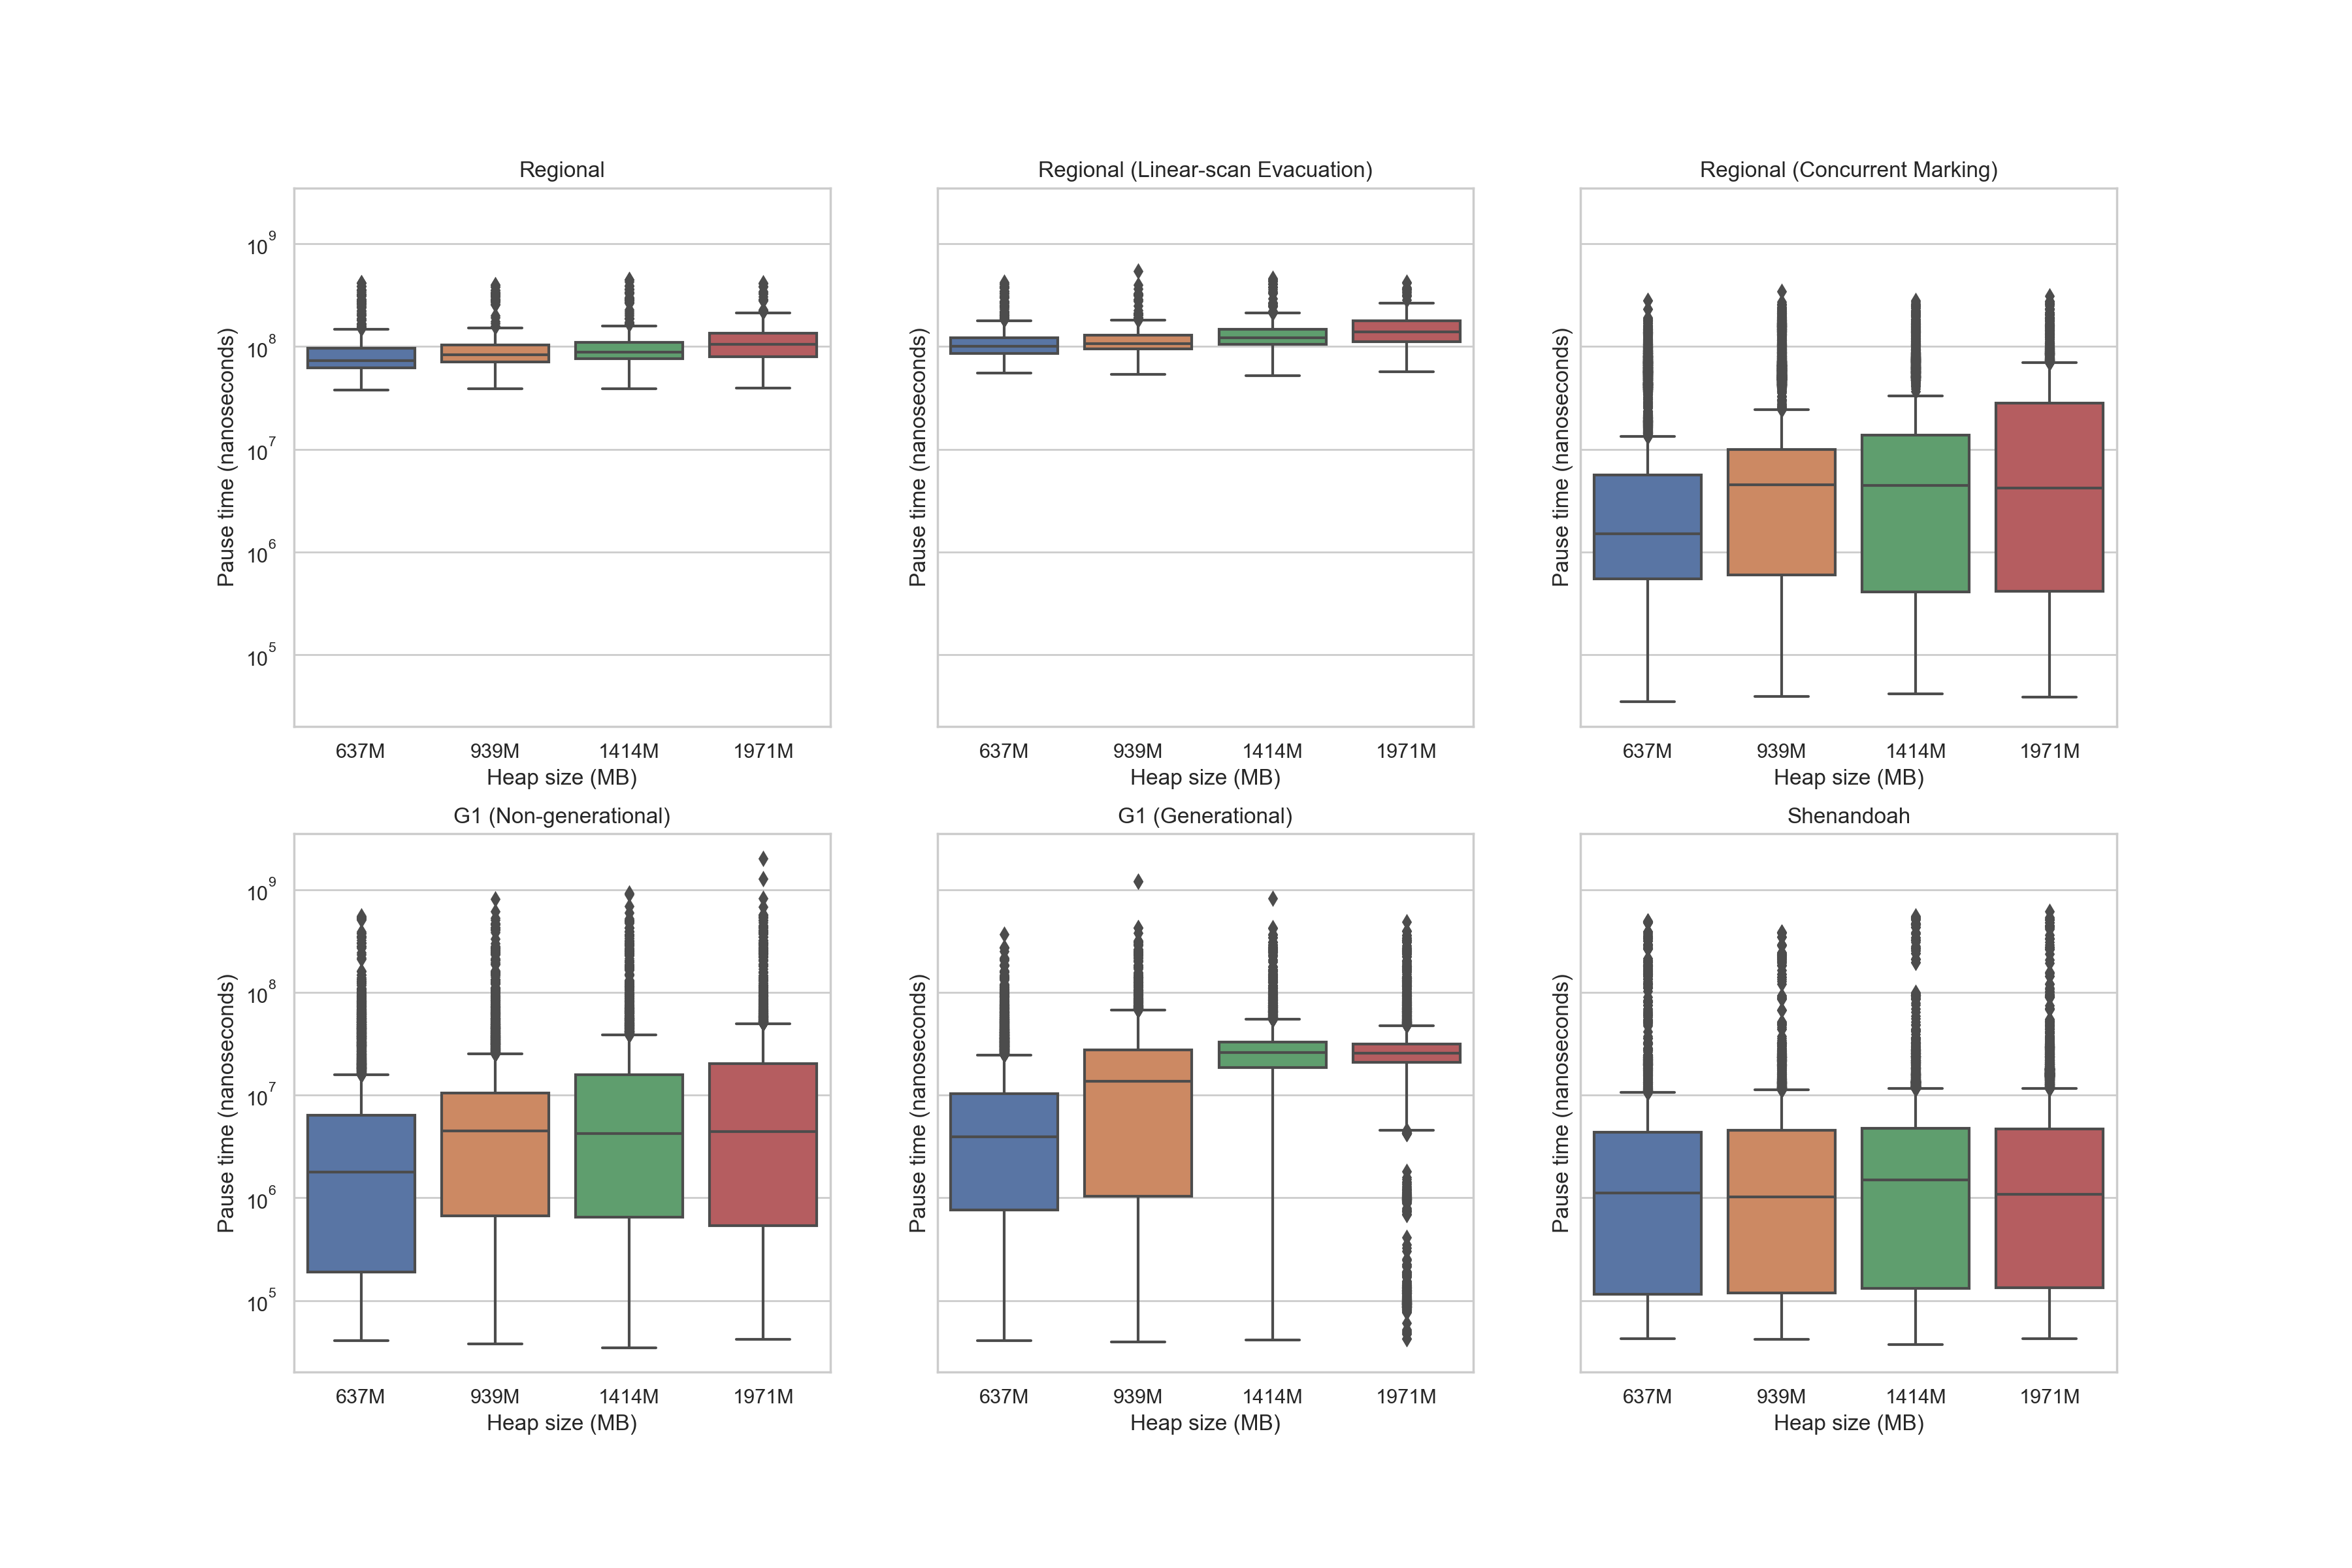
\includegraphics[width=\textwidth/1]{{figs/pause-time.png}}
  \caption{Pause times of 6 collectors}
  \label{fig:pausetime}
\end{figure*}

\begin{table*}
  \centering
  \input table/full-gc-ratio.tex
  \caption{Ratio of full gc}
  \label{tab:remsetfootprint}
\end{table*}

Figure~\ref{fig:pausetime} shows the results of the GC latency time
evaluated on all 6 garbage collectors discussed in section~\ref{cha:implementation}.
Each subfigure shows
the overall GC latency time for each garbage collector. Specifically, the
minimum, 25\% percentile, medium, 75\% percentile and maximum GC latency time nanoseconds
were reported for each collector and each heap size.

To present the results more clearly, the benchmarking results ar presented as
a set of box plots and with log-scaled pause time y in nanoseconds as y-axis.

\subsection{Discussion}

As the most simple form of the G1 family of GC, the Regional collector, performs fully
stop-the-world GC during each GC cycle. Works for each GC cycle includes marking all
live objects and walk over the object graph to evacuate objects in a set of selected memory
regions. Totally 2 full heap tracing are performed during each GC cycle, which makes the GC
pause time longer. The average pause time for this Regional GC generally ranges from $104$ to $147$
milliseconds and inceases as the heap size inceases.

By performing linear scan based evacuation, the linear-scan evacuation version of the Regional
GC has to scan the memory regions in the collection set twice, one for exacuating live objects and
one for updating references. In this way the collector generally has longer pause times,
which ranges from $139$ to $198$ milliseconds in average and and inceases as the heap size inceases.
The percentage of GC pause time increase are 33.7\%, 30.5\%, 26.9\%, 34.8\% for 4 heap sizes
respecively, in average 31.5\%.
Although performing linear scan evacuation can largely increases the GC pause time,
this indenpendent phase is a important part for G1 GC and the Shenandoah GC.

After performing concurrent marking in additional to the linear scan based evacuation,
the resulting ConcRegional collector split the pause for marking into several smaller
pauses and performs most of the marking work in concurrent without stopping the mutators.
This makes the total pause time for a GC smaller and significantly reduces the average
pause time by 88.5\%.

The non-generational G1 reduces the collection size to meet a pause time goal of 100\,ms.
Based on the benchmarking results, at least 75\% of the pauses are less than the pre-defined
pause time goal. On the other hand, G1 uses remembered sets to update references
instead of performing full heap tracing.
To small heaps this has almost no benefits, even reduces the average pause time by
24.9\% on 637\,MB heaps. But for heap sizes of 39\,MB, 1414\,MB and 1971\,MB, this
partial heap scanning technique reduces average pause time by 8.8\%, 7.4\% and 10.7\%
respecively. So the remembered sets based references updating has more benefits on
larger heaps. However, the full GC becomes more expensive because of the large work required
to update all the remembered sets in the heap, which usually results in a pause time
ranges from 0.5\,s to 1.5\,s.

By using the generational G1 GC, young/nursery GCs are usually triggered several times
before a major GC happens. Also nursery GCs are fully stop-the-world and always tries
to collect as much nursery regions as possible, as long as the pause time does not exceeds
the pre-defined pause time goal. This results in the incease of GC pause times.
\pending{Any benefits ??????}

The Shenandoah GC performs marking, evacuation and reference updating in concurrent,
this significantly reduces the pause time by 72.6\%, compared to the concurrnet marking version
of the regional collector. Based on the benchmarking results at least 75\% of
the GC pauses do not exceeds 10 milliseconds. However, full GCs can still results
in pauses of around 500 to 600 milliseconds, which is longer than the concurrent-marking
regional collector due to the Brooks barrier involved during evacuation, which performance
will be discussed in section~\ref{sec:barrierlatency}

\section{Barrier Latency Evaluation} % 7
\label{sec:barrierlatency}

This section describes the steps took for barrier overhead evaluation as well as
all the evaluation results and discussions.

\subsection{Methodology}

The mutator barrier percentage overhead is modelled as follows:
$$
\text{Overhead} = \frac{|\text{Mutator time with barrier} - \text{Mutator time without barrier}|}{\text{Mutator time without barrier}} * 100\%
$$

The mutator execution time is calculated as the execution time of the benchmarking program with
stop-the-world gc time excluded.

As discussed in chapter~\ref{cha:implementation}, I implemented the Garbage-first
family of collectors by performing progressive improvements on a simple region-based collector.
In this way, after performing an algorithmic improvement on a collector, we can measure the overhead of
the newly involved barriers or other technologies by comparing the benchmarking results
of the old collector and the new collector.

As an output of the analysis of the overhead data, the average barrier overhead
for each GC, each benchmark suite, each heap size and each barrier this project used is reported
as well as their corresponding 95\% confidence interval.
The overall average overhead and 95\% confidence interval for each barrier is also reported.

\subsection{Snapshot-at-the-begining barriers}

\begin{table*}
  \centering
  \input table/satb-barrier.tex
  \caption{Snapshot-at-the-begining barrier overhead}
  \label{tab:satbbarrier}
\end{table*}

Table~\ref{tab:satbbarrier} shows the overheads of the Snapshot-at-the-begining barrier
as well as their 95\% confidence interval on different heap sizes.

\pending{Discussion}

\subsection{Remembered set barriers}

\begin{table*}
  \centering
  \input table/remset-barrier.tex
  \caption{Remembered set barrier overhead}
  \label{tab:remsetbarrier}
\end{table*}

Table~\ref{tab:remsetbarrier} shows the overheads of the Remembered set barrier
as well as their 95\% confidence interval on different heap sizes.

\pending{Discussion}

\subsection{Brooks indirection pointer barriers}

\begin{table*}
  \centering
  \input table/brooks-barrier.tex
  \caption{Brooks indirection pointer barrier overhead}
  \label{tab:brooksbarrier}
\end{table*}

Table~\ref{tab:brooksbarrier} shows the overheads of the Brooks indirection pointer barrier
as well as their 95\% confidence interval on different heap sizes.

\pending{Discussion}

\section{Remembered-Set Size} % 7
\label{sec:remsetsize}

\subsection{Evaluation metrices}
\subsection{Results}

\begin{table*}
  \centering
  \input table/remset-size.tex
  \caption{Remembered set footprint}
  \label{tab:remsetfootprint}
\end{table*}

\subsection{Discussion}

\section{Summary} % 2
\label{sec:summary}

This chapter discusses the measurement methodology and results for evaluating the
performance of the G1 family of garbage collectors. This includes the evaluation of
GC pause times and overhead of several mutator barriers. Also the phenomenon revealed
in the measurement results is carefully discussed.

On the one hand, based on the measurement results, we can see that linear scan based evacuation
increses the work for each GC. Using concurrent marking, concurrent evacuation
or remembered set based partial heap scanning can significantly reduces the pause time
for each GC. On the other hand, using mutator barrier barriers can largely increase the
mutator throughput reduction.

Also based on the measurement results, the generational G1 and Shenandoah GC shows some
disappointing performance on GC pause time and mutator overheads respecively.
However, the time scope of this project is limited.
In this way, there are still much optimization job and other work to do in the future,
which will be discussed in Chapter~\ref{cha:conc}.




%%% Local Variables: 
%%% mode: latex
%%% TeX-master: "paper"
%%% End: 


% We can also refer to specific lines of code in code listings. The bug in
% \Cref{fig:c:hello} is on \cref{line:bug}. There is also a bug in
% \Cref{fig:java:hello} on \crefrange{line:jbug-start}{line:jbug-end}. To
% achieve these references we put
% \texttt{(*@ \textbackslash label\{line:bug\} @*)}
% in the code -- the \texttt{(*@ @*)} are escape delimiters that allow you to add
% LaTeX in the (otherwise verbatim) code file.

% \begin{table*}
%   \centering
%   \caption{Processors used in our evaluation.  Note that the caption for a table is at the top.  Also note that a really long comment that wraps over the line ends up left-justified.}
%   \label{tab:machines}
%   \input table/machines.tex
% \end{table*}

% \begin{figure}
%   \centering
%   \begin{subfigure}[b]{\textwidth}
%       \lstinputlisting[linewidth=\textwidth,breaklines=true]{code/hello.c}
%       \caption{C}
%       \label{fig:c:hello}
%   \end{subfigure}

%   \begin{subfigure}[b]{\textwidth}
%       \lstinputlisting[linewidth=\textwidth,breaklines=true]{code/hello.java}
%       \caption{Java}
%       \label{fig:java:hello}
%   \end{subfigure}

%   \caption{Hello world in Java and C. This short caption is centered.}
%   \label{fig:helloworld}
% \end{figure}